\section{Introduction}

    Many programs fall victim to having lots of redundant code.
    Right from simple redundant writes to outright dead code, removing them plays a major role in performance of our programs. 
    Such redundancy could also be possible due to different phases of optimization the compiler performs, which leaves certain residual code in each phase.
    Examples of such optimizations are common-sub-expression elimination, copy propagation, partial redundancy elimination, register allocation, etc.
    
    In a sequential setting the effect of removing such code can be addressed easily.    
    However, as we saw for instruction reordering, in a concurrent setting, elimination may not be that straightforward. 
    Consider the first example in Figure~\ref{elim:example1(a)} below of a Candidate(left) and the resultant candidate after eliminating a write(right).
    The orange box shows the observable behavior that we want to consider. 
    \begin{figure}[H]
        \centering
        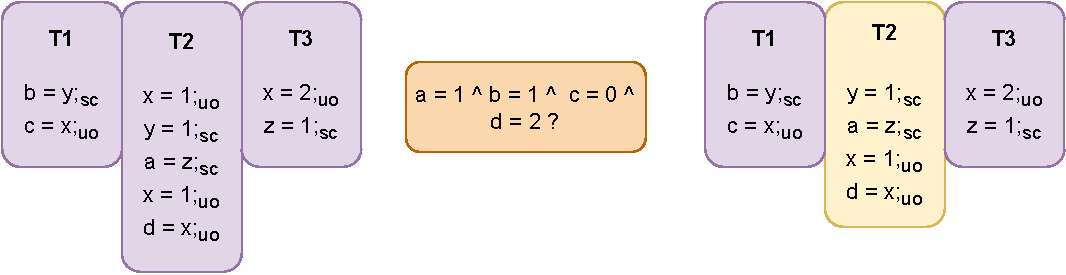
\includegraphics[scale=0.7]{6.Elimination/EliminationExample1(a).pdf}
        \caption{First example for elimination with candidates of the original program and its counterpart after elimination of a write.} 
        \label{elim:example1(a)}
    \end{figure}

    Figure~\ref{elim:example1(b)} explains the relations formed in a candidate execution that disallow the behavior in question for the original program but justify it after elimination. 
    The first set of relations is for the original program, where Axiom \ref{CoRe} prohibits the read $d$ to have value of $x$ as $2$.
    The second set is for the modified program, where none of the axioms restrict such a behavior (I would suggest the avid readers to check it for themselves).
    \begin{figure}[H]
        \centering
        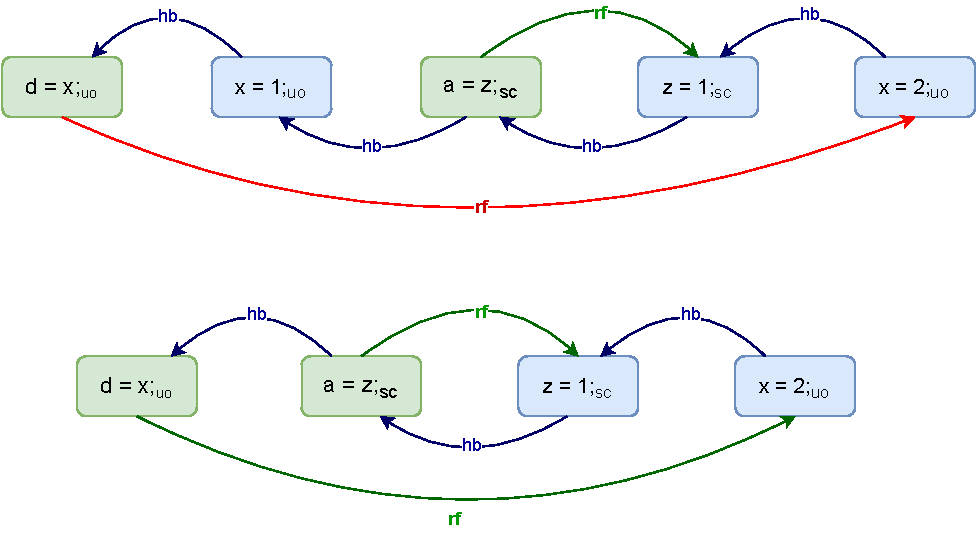
\includegraphics[scale=0.7]{6.Elimination/EliminationExample1(b).pdf}
        \caption{The set of partial order relations justifying the observable behavior in question for both the candidates in Figure~\ref{elim:example1(a)}.} 
        \label{elim:example1(b)}
    \end{figure}

    In the case of read elimination, we clearly would lose observable behaviors w.r.t. to the read eliminated.
    However, our focus is more on whether eliminating this read introduces new observable behaviors in the remaning program, meaning, can other reads be affected.
    Constructing such an example is non-trivial and involves implied memory order edges that are created between events.
    Figure~\ref{elim:example2(a)} shows such an example where the Original Candidate (left) and the one after eliminating a read in $T2$ is shown.
    The orange box represents the behavior in question. 
    \begin{figure}[H]
        \centering
        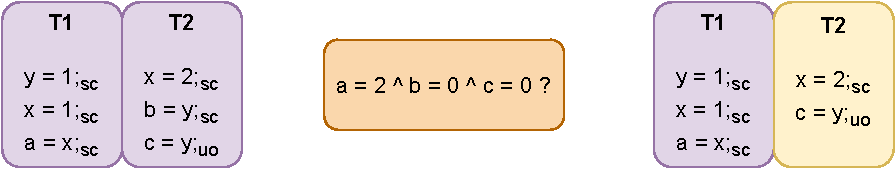
\includegraphics[scale=0.7]{6.Elimination/EliminationExample2(a).pdf}
        \caption{First example for elimination with candidates of the original program and its counterpart after elimination of a read.} 
        \label{elim:example2(a)}
    \end{figure}

    Figure~\ref{elim:example2(b)} explains the relations formed in a candidate execution that disallow the behavior in question for the original program but justify it after elimination. 
    In the first set of relations, the read $a$ to have value of $x$ as $2$ implies a memory order between $x=1$ and $x=2$. 
    This then, by Axiom \ref{SeqCsAt} prohibits the read $b$ to have value of $y$ as $0$.
    This in turn results in a happens-before relation, which then by Axiom \ref{CoRe} prohibits the read $c$ to have value of $y$ as $0$.
    The second set is for the modified program, where none of the axioms restrict such a behavior\footnotemark. 
    This hints towards the fact that the read value of $a$ itself restricts the value of $c$, which we cannot capture without the presence of read $b$.
    \begin{figure}[H]
        \centering
        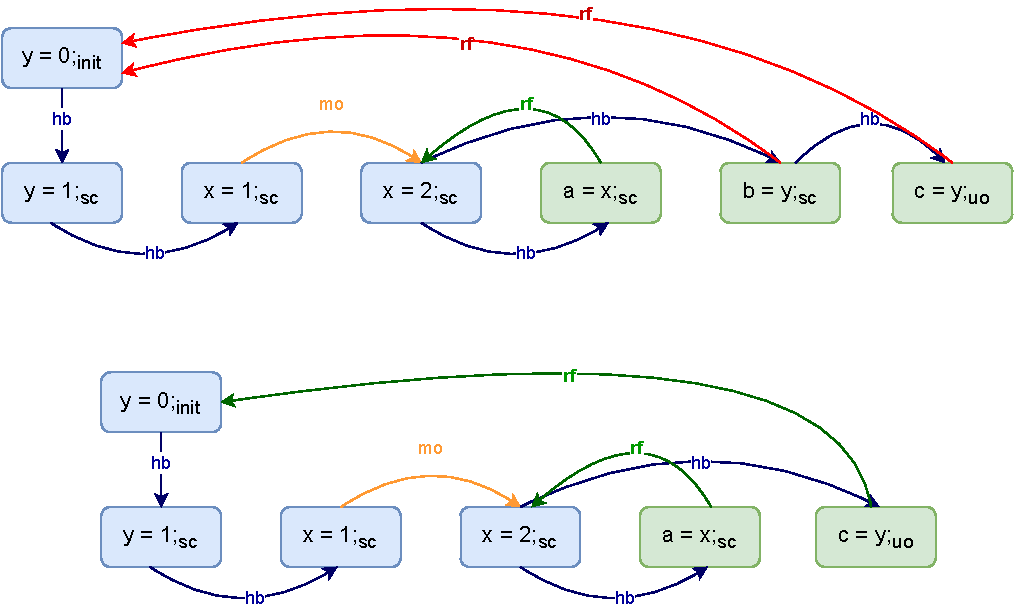
\includegraphics[scale=0.7]{6.Elimination/EliminationExample2(b).pdf}
        \caption{The set of partial order relations justifying the observable behavior in question for both the candidates in Figure~\ref{elim:example2(a)}.} 
        \label{elim:example2(b)}
    \end{figure}
    
    \footnotetext{The avid reader may note that as long as the read value of $a$ is $2$, the value of $c$ can never be $0$. But as we eliminate $b$, none of the axioms disallow the behavior in question.}